\documentclass[11pt]{article}
\usepackage[margin  = 1in]{geometry}
\usepackage{hyperref}
\bibliographystyle{ieeetr}
\usepackage{amsmath} 
\usepackage{graphicx}
\usepackage{float}
\usepackage{subcaption}
\bibliographystyle{ieeetr}

\begin{document}

\title{Optimizing Terahertz Leaky Wave Antennas Using Deep Learning Predicted Periodically  Modulated Slots}
\author{J. Neronha, H. Guerboukha, and D. Mittleman \\ \\ \small School of Engineering, Brown University, Providence, RI 02912}
\date{}

\maketitle

\section*{Introduction}

The predictive power of neural networks and machine learning techniques more generally have been applied to a vast array problems ever since the neural network was proposed as a computational technique loosely modeling the brain in the mid-twentieth century. \cite{McCulloch:1943vq} This, of course, includes communications technology -- neural networks have been used extensively in the field because of their unique ability to approximate accurate solutions to nonlinear problems that are commonplace in antenna design. Machine learning models are particularly useful in situations where an analytical solution cannot be obtained and/or numerical simulations are expensive \cite{Kim, Massa}. These types of problems are usually split into two cases, forward and inverse problems. The former refers to situations where models attempt to generate the electromagnetic response given some parametric input, while the latter attempts the reverse: predicting those parameters given some signal \cite{9395365}. \\

\noindent Examples of direct problems include approximating an antenna's output given a geometry \cite{8608745} or modeling a metasurface \cite{Nadell:19}, which could take a finite-element model hours or longer to solve, limiting real-time simulation and design. Inverse problem considers the opposite direction, for example reconstructing an image from scattered light \cite{Sun:18}. There have been many applications of neural networks to communications-related problems, for example, in the optimization of massive multiple-input multiple-output (MIMO) systems to improve signal reconstruction quality \cite{8322184} or physical layer design \cite{DBLP:journals/corr/OSheaEC17}. \emph{MORE EXAMPLES HERE?} \\

\noindent We are particularly interested in the inverse problem of terahertz leaky-wave antenna (LWA) design because of its high applicability to the field of communications -- given some arbitrarily desired far-field pattern, how can we quickly design, fabricate, and test an antenna that meets our needs? Periodic leaky wave-antennas are especially interesting for signal design because of their characteristic emissions at various angles, both forward and backwards scattering, that depend on the periodicity, allowing for a wide variety of potential peak angles \cite{6556051}. And while traditional communications systems demand broad angular emission, the terahertz range (i.e. $>$ 100 GHz) requires focusing power along narrow directional beams due to substantial power loss as a result of free path losses at higher frequencies \cite{doi:10.1063/1.5014037, Ghasempour:2020tz}, meaning that highly specific peak profile design is crucial. \\

\noindent LWAs are simple metallic waveguides that have proven very effective in the terahertz range and are particularly interesting because they emit radiation at a frequency-dependent angle with a one-to-one relationship between frequency and angle, which is quite valuable given the narrow character of beams in the terahertz range. \cite{doi:10.1063/5.0033126} They have been used in a number of diverse applications including link discovery \cite{Ghasempour:2020tz}, multiplexing and demultiplexing \cite{Karl:2015uh, Ma:2017vo}, and for radar and object detection purposes \cite{Amarasinghe:20, Amarasinghe:21}. Leaky-wave antennas also stand out for our purposes of rapid design and experimentation because of the ease of fabricating them using hot-stamping techniques \cite{Guerboukha:21}. This inverse problem has been explored in the terahertz range using deep neural networks in the context of designing structures to obtain an optimized geometry that produces the desired signal, particularly in relation to metasurface design \cite{Deng:21, 9602997}. The inverse Leaky-wave antenna problem has also been explored, but using a genetic algorithm and outside of the terahertz range at much higher frequencies \cite{Jafar-Zanjani:2018vy}. \\

\noindent As a result, in this paper, we propose a model to predict the ideal LWA geometry that will generate desired far-field radiation in the terahertz range. Specifically, we suggest an antenna design where a LWA is broken into sub-slots, each of which can either be metallic, transparent, or somewhere in between (i.e. partially transparent). Thus, we find that any slot composed of an array of these sub-slots forms a linear superpositioning of periodic modes that can be used to generate highly specific peak profiles.

\section*{Methodology}

We train a model to predict the slot geometry of the LWA for a desired far-field pattern. We consider a LWA based on a parallel plate waveguide, the fundamental transverse electric (TE$_1$) mode, and a frequency of 200 GHz. Instead of a uniform 1D slot \cite{doi:10.1063/5.0033126}, we discretize the slot into 36 0.5-mm sub-slots that can be transparent, metallic, or somewhere in between (i.e. semi-transparent). This approach is similar to the approach taken in past explorations of metasurface design \cite{Liu:2022tg, Jafar-Zanjani:2018vy}. According to Floquet theory \cite{6556051}, a periodic array of slots excites an infinite number of space harmonics each with its distinct dispersion constant $\beta_p$:

\[\beta=\sqrt{k_0^2 - (\frac{\pi}{h})^2} +\frac{2\pi p}{\Lambda} \tag{1} \label{eq:special}\] 

\noindent where $k_0$ is the wave number, $h$ is the height of the waveguide, and $\Lambda$ is the slot periodicity. These different modes peak at different angles defined by $\cos(\theta)=\beta_p/k_0$, given that the excited modes can be consider fast-wave (i.e., $|\beta_p|>k_0$). Our primary objective is to generate multiple beams with specific magnitudes at specific locations. Therefore, instead of a periodic geometry, we consider a non-periodic array of slots. By Fourier decomposition, we note that any non-periodic slot design can be viewed as a linear combination of periodic designs $\beta_p$, each peaking at an angle $\cos(\theta)=\beta_p/k_0$. The strength (amplitude) of individual peaks can be related to the Fourier coefficients of this decomposition. \\

\noindent Our discretized geometry imposes limits on the possible excited Floquet modes, by constraining the values of $\Lambda$. Indeed, due to the discretization, the possible $\Lambda$ are given by $\Lambda=$. Furthermore, due to the fast-wave requirement (i.e., $|\beta_p|>k_0$), only a few select modes will be able to leak out of the waveguide. We propose two different schemes for generating a desired signal:

\begin{enumerate}
	\item each sub-slot can be either transparent or metallic (left panel of Figure 1)
	\item each sub-slot can also take some intermediate value of opacity (right panel of Figure 1)
\end{enumerate}  

\noindent A schematic of both schemes is shown in Figure 1 below. Additionally, Figure 2 shows all possible peaks from the various modes and periodicities Floquet theory and these peaks overlaid a sample far-field signal from a similar geometry.

\begin{figure}
		\centering
		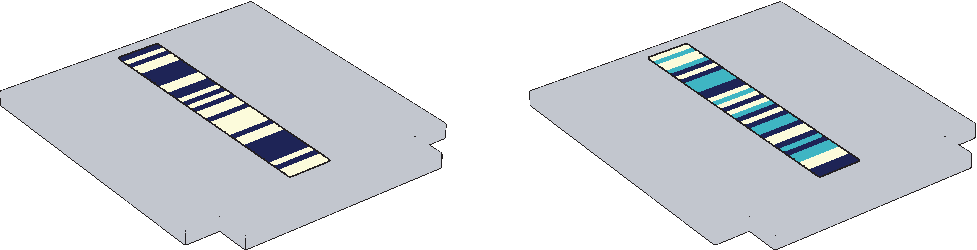
\includegraphics[height=1.5in]{figures/fig5pdf}
		\caption{The leaky wave antenna geometry. The left panel shows the binary case, where dark-colored sub-slots represent transparent areas while light colors indicate metallic boundaries. In the right panel, the boundary conditions are no longer discretized and can take on some intermediate value of transparency, as seen by the sub-slots with colors between light and dark.}
\end{figure}


\bibliographystyle{plain}
\bibliography{references.bib}
\end{document}